
% Packages
\documentclass[11pt,a4paper]{article}
\usepackage[utf8x]{inputenc}
\usepackage[T1]{fontenc}
\usepackage{mathptmx}


\usepackage[pdftex]{graphicx}
\usepackage[pdftex,linkcolor=black,pdfborder={0 0 0}]{hyperref}
\usepackage{calc}
\usepackage{enumitem}

\frenchspacing

% Set linespace
\linespread{1.2}

%margins
\usepackage[a4paper, lmargin=0.1666\paperwidth, rmargin=0.1666\paperwidth, tmargin=0.1111\paperheight, bmargin=0.1111\paperheight]{geometry}

% Tries to remove widows
\usepackage[all]{nowidow}

% Improves typography, load after fontpackage is selected
\usepackage[protrusion=true,expansion=true]{microtype}

\usepackage{lipsum}

% package for authors
\usepackage{authblk}

% add graphics dir
\usepackage{graphicx}
\graphicspath{ {../figures/} }
\usepackage{wrapfig}
\usepackage[export]{adjustbox}

% Begin document
\begin{document}

\begin{titlepage}

    \title{KEGGTOOLS - Toolkit for enrichment and visualization of KEGG pathways}

    \author[1]{Malte Hellmig}
    \author[1, 2]{PD Dr. med. Christian Krebs}
    \author[1, 2]{Prof. Dr. med. Ulf Panzer}
    \affil[1]{\small{\textit{III. Department of Medicine, Division of Translational Immunology, University Medical Center Hamburg-Eppendorf, Hamburg, Germany.}}}
    \affil[2]{\small{\textit{Hamburg Center for Translational Immunology (HCTI), University Medical Center Hamburg-Eppendorf, Hamburg, Germany.}}}
    \date{}
    \clearpage\maketitle
    \thispagestyle{empty}


    \section*{Abstract}

    The enlargement of transcriptomic datasets due to high-throughput methods
    like single cell RNA sequencing desire for reproducible analysis as well
    as understandable and expressive visualisations. A way to address complex
    information in this field is the enrichment analysis. KEGGTOOLS is a
    Python-based package to efficiently compute and plot enrichment of a given
    gene list based on the pathway database of the Kyoto Encyclopedia of Genes
    and Genomes. The package is published and freely available on Github:
    \mbox{\url{https://github.com/harryhaller001/keggtools}}.


\end{titlepage}

% start new page and set page counter to 1
\newpage
\setcounter{page}{1}

\section{Introduction}

\lipsum[1-2]


% \begin{figure}

% % 1142x1858 px
% 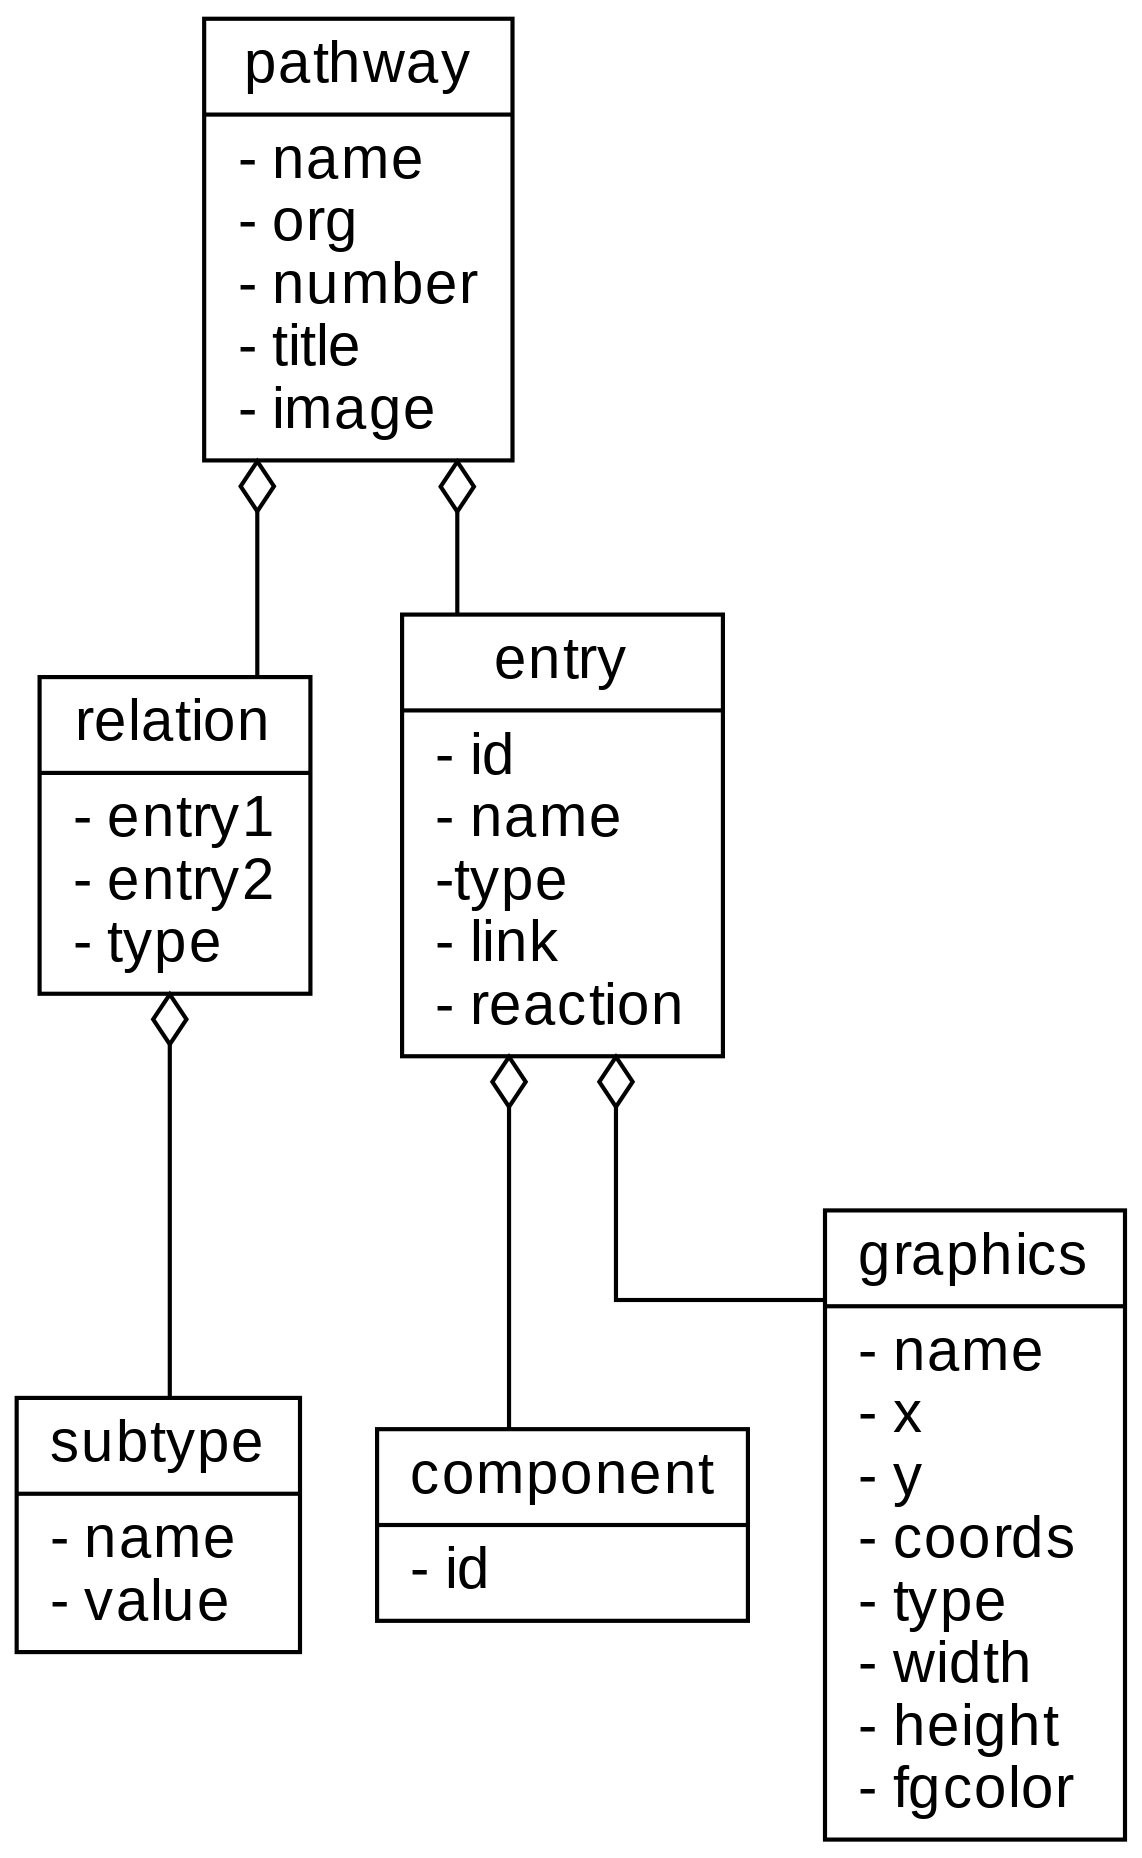
\includegraphics[width=5cm]{figure1.png}

% \caption{Figure 1: Object structure of KEGG database models}
% \end{figure}


% figure of KEGG database structure
\begin{wrapfigure}{l}{0.5\textwidth}

    % 1142x1858 px
    \centering{
        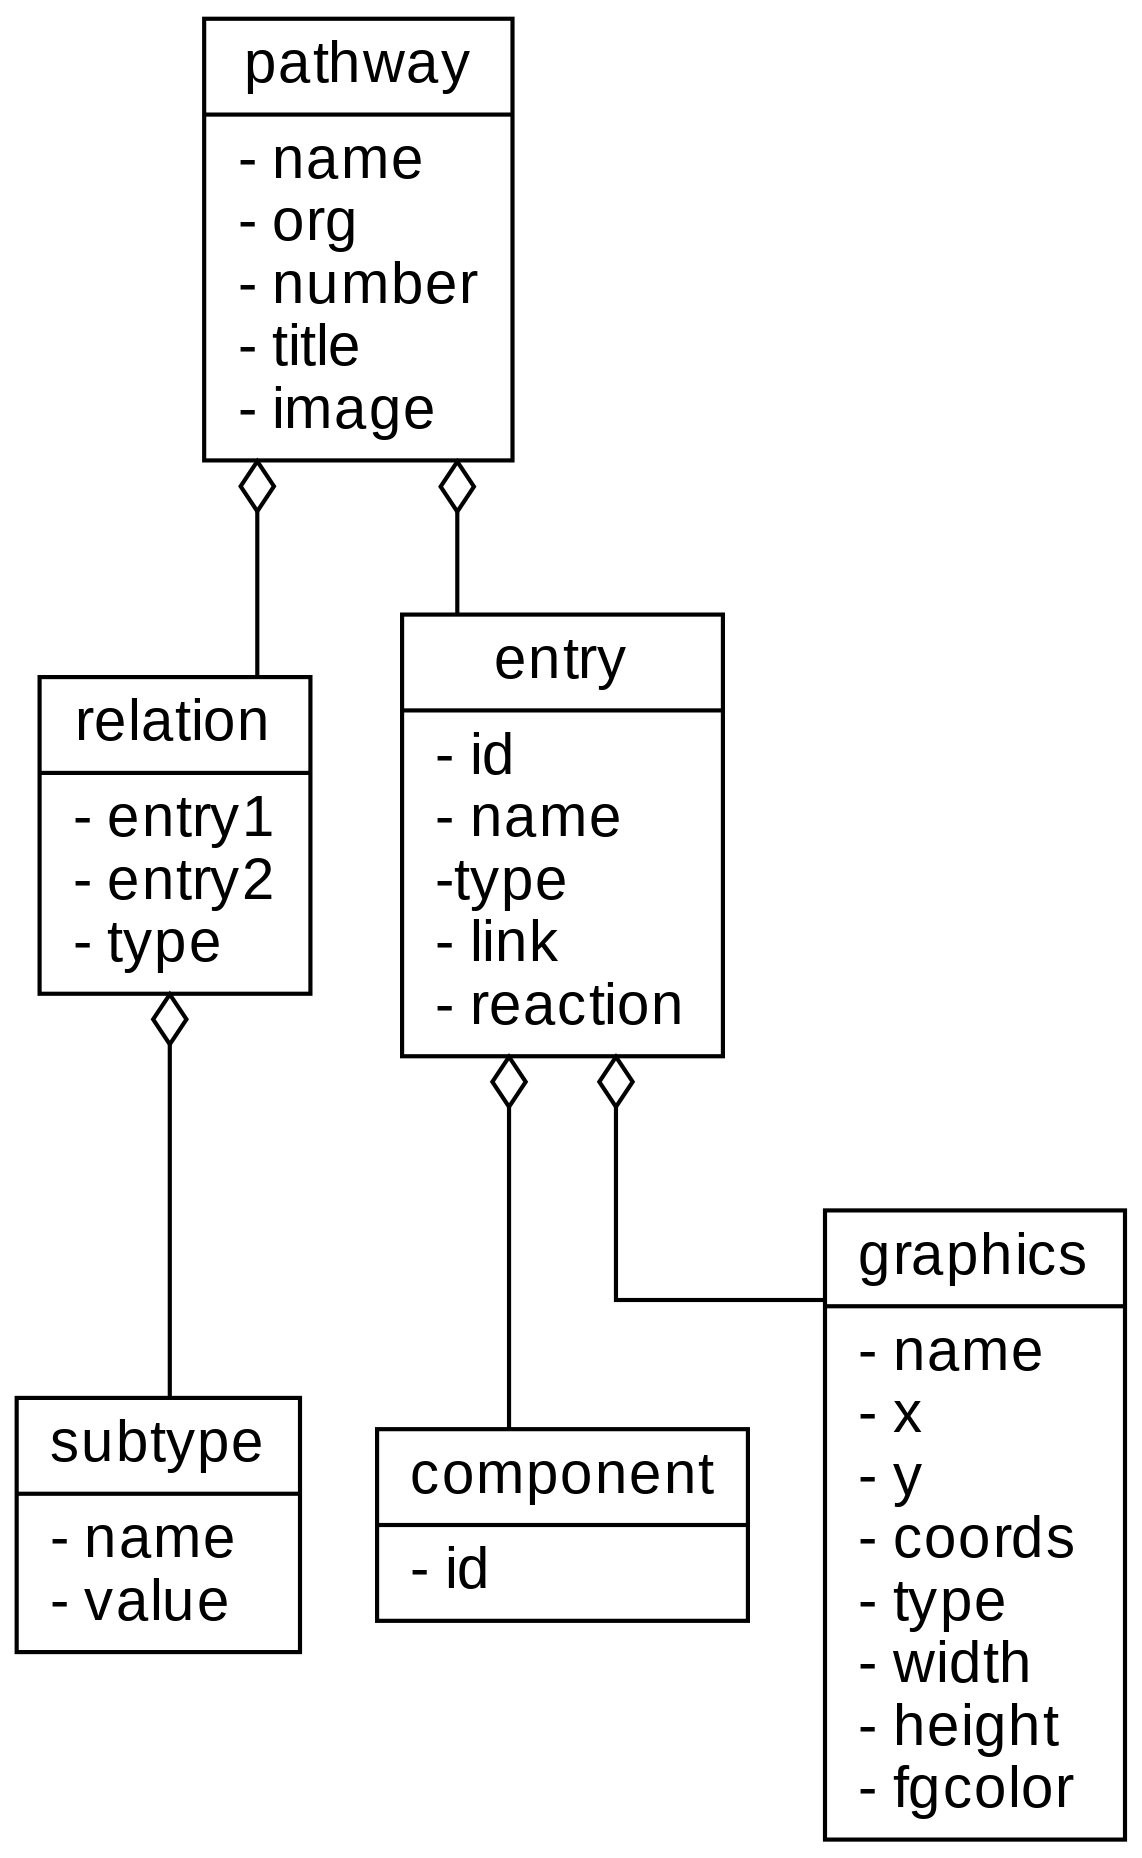
\includegraphics[width=5cm]{figure1.png}
    }

    \caption{Object structure of KEGG database models}
\end{wrapfigure}

\lipsum[3-4]


% Figure of single cell analysis
\begin{figure}

    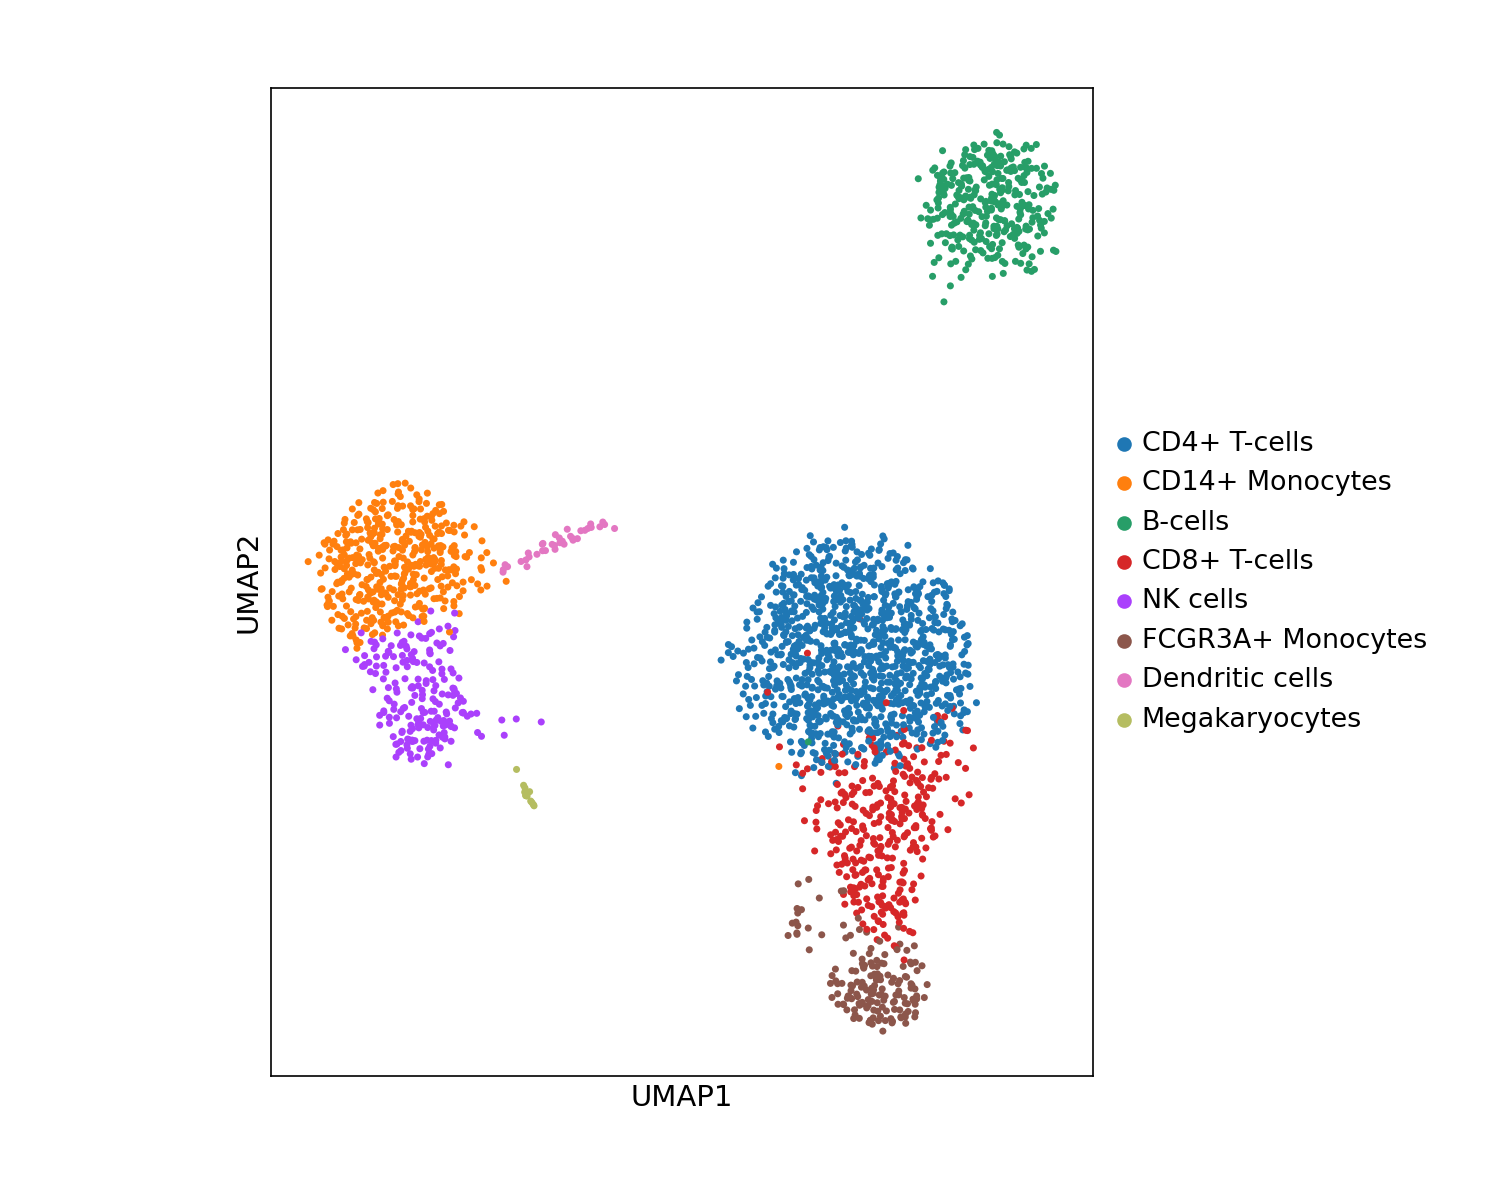
\includegraphics[width=0.5\textwidth, valign=t]{figure2.png}
    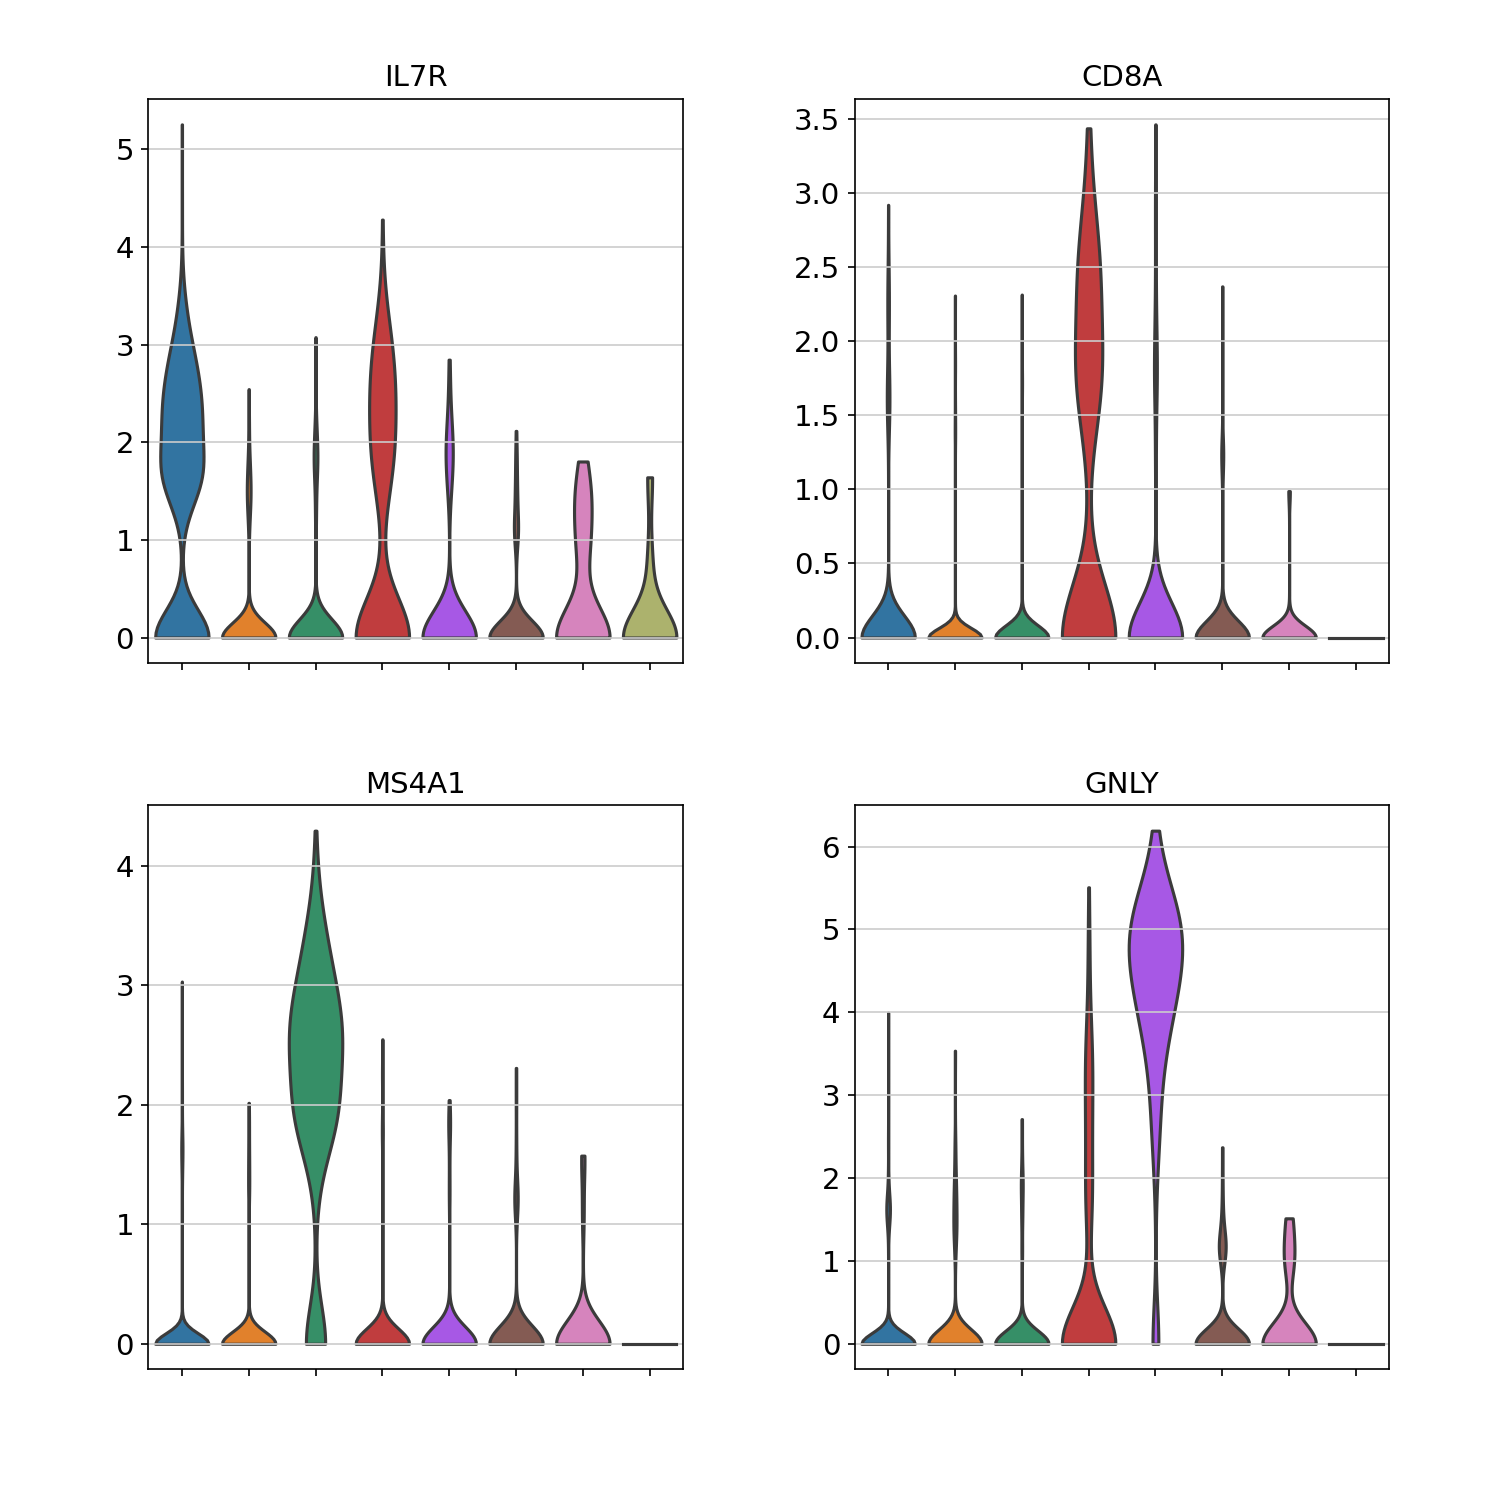
\includegraphics[width=0.5\textwidth, valign=t]{figure3.png}

    \caption{Analysis of the single cell RNA dataset PBMC3K. It show the cell distribution in the UMAP space with
    cluster annotation (left) and identified marker genes (right).
    }
\end{figure}



\subsection*{Subtitle}
\lipsum[4-5]
\end{document}

